\label{sec:sysml:analysis}

\subsection{Model and Task Variations}
\begin{comment}
\begin{figure*}[!!htbp]
    \begin{subfigure}{0.5\textwidth}
        \centering
        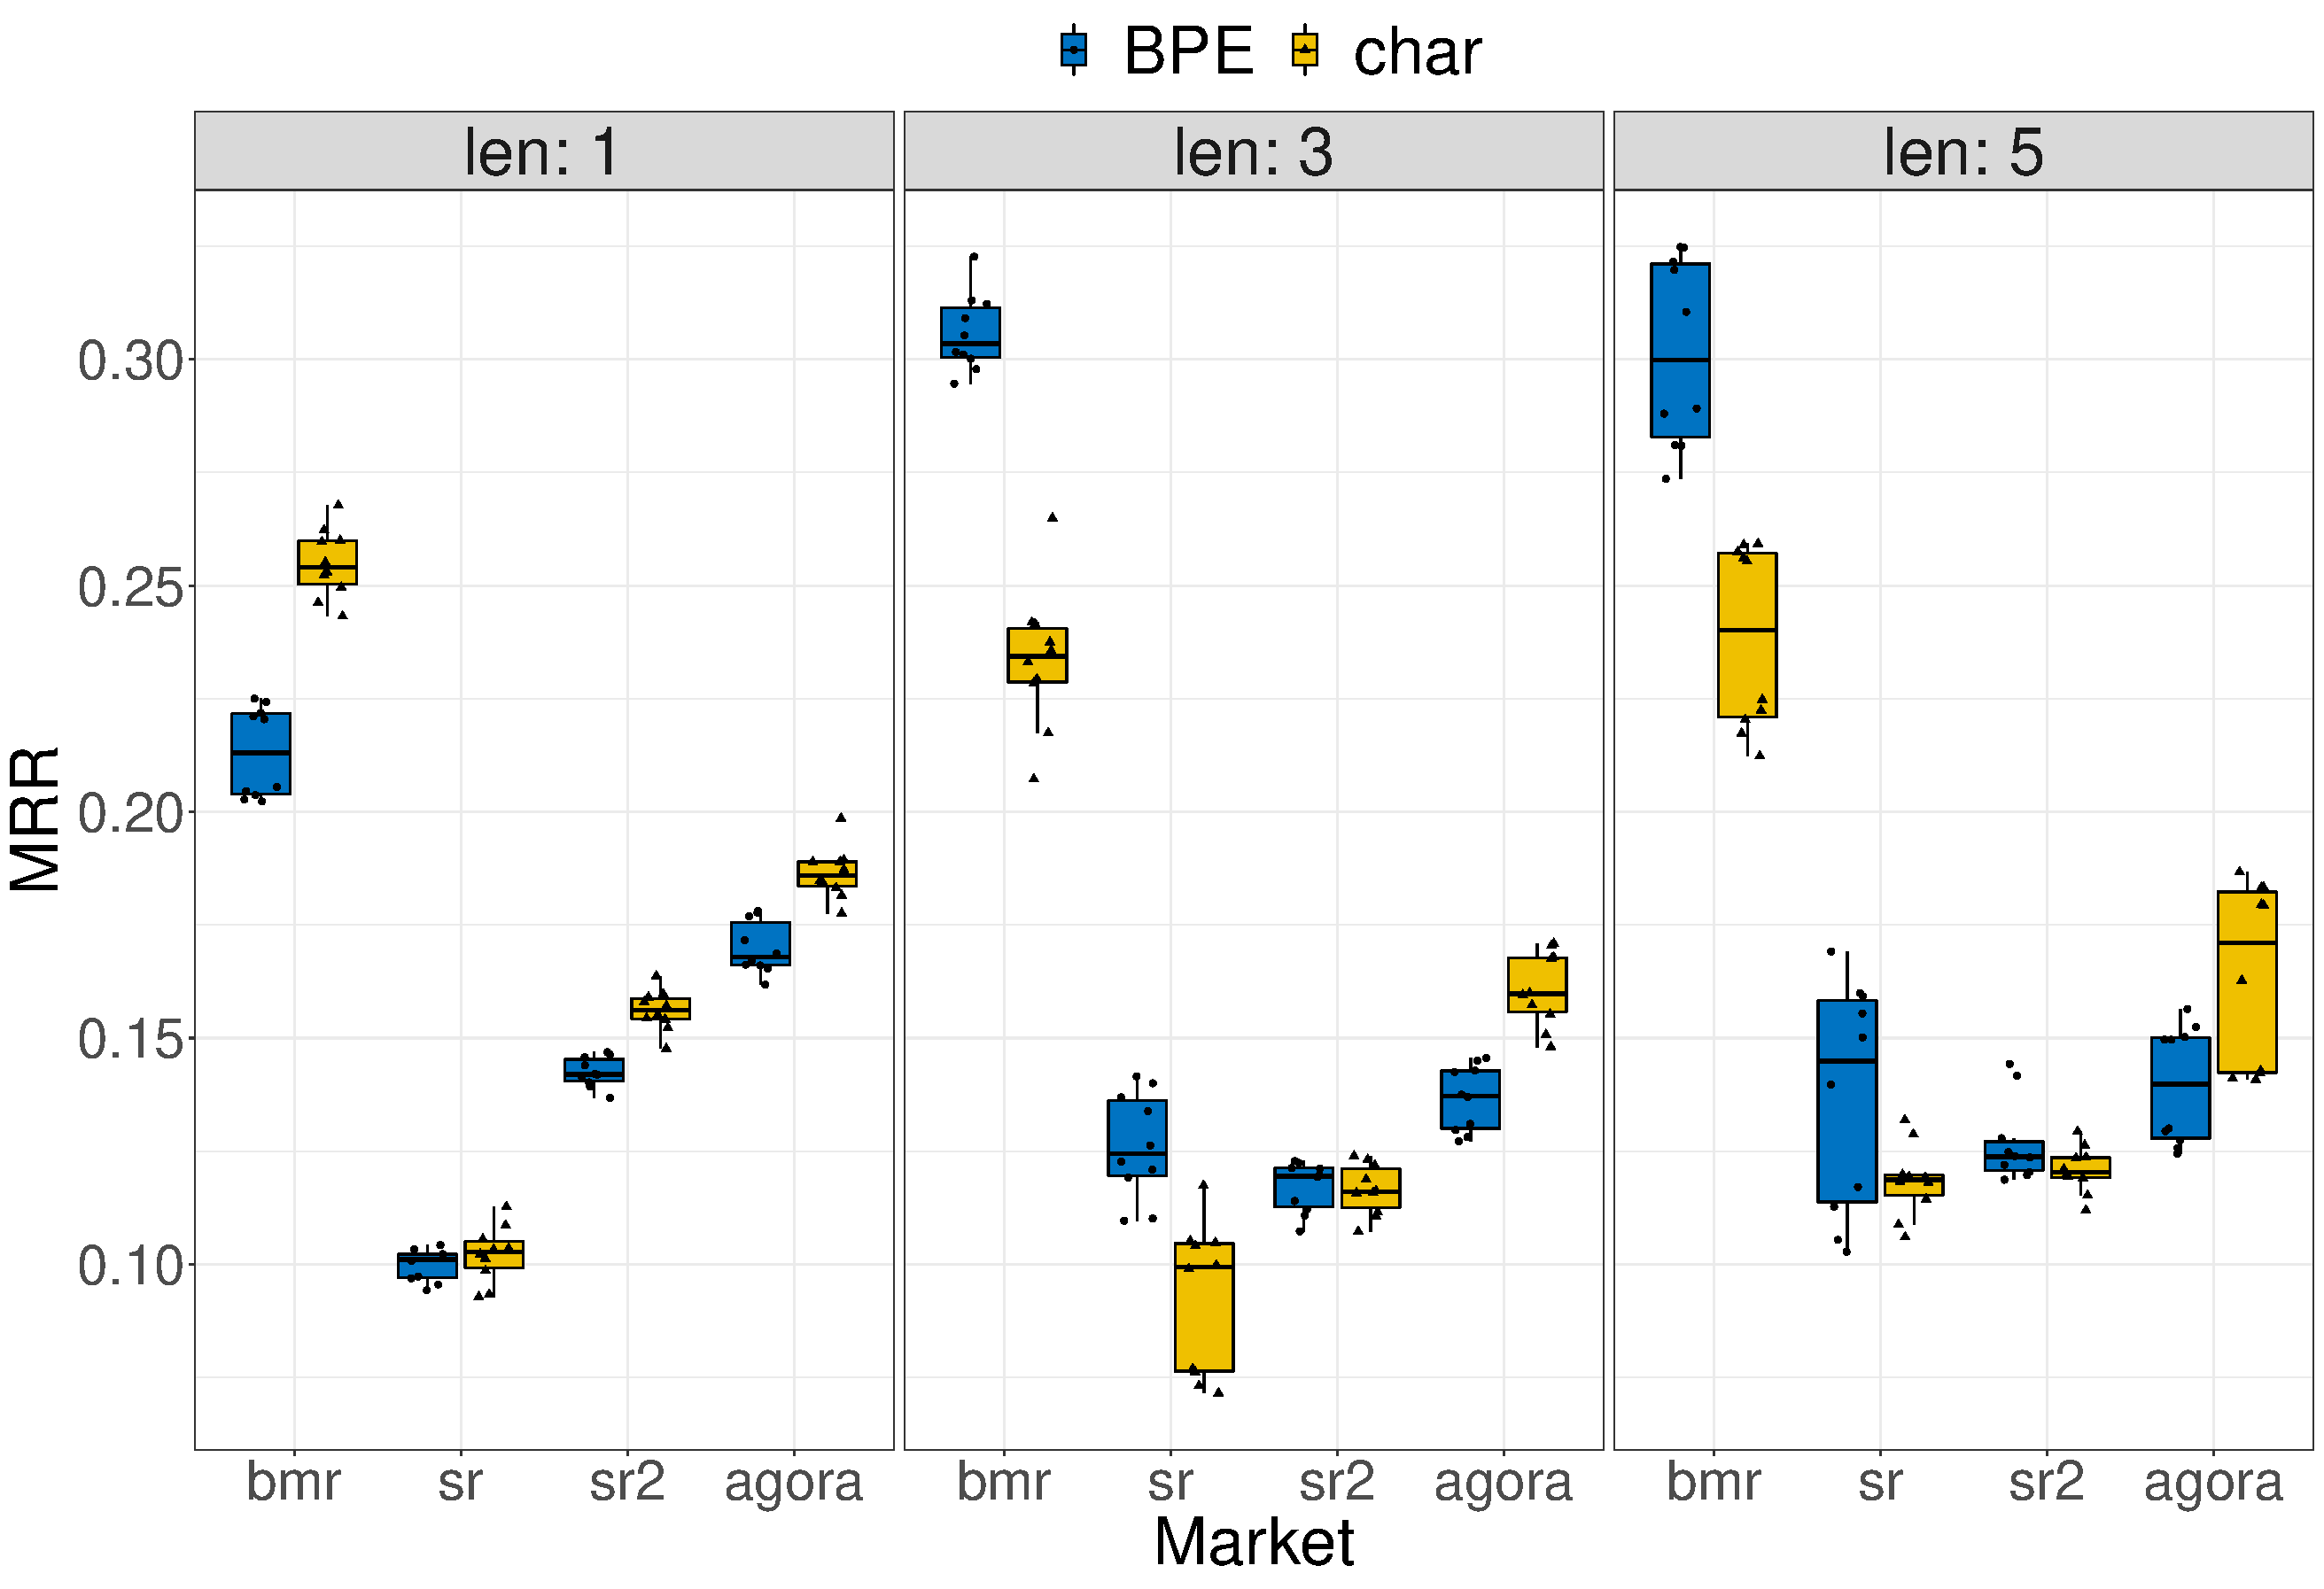
\includegraphics[width=\linewidth]{plots/tokenizer_comparison.pdf}
        \caption{Tokenizer}
        \label{fig:model_comp:tok}
    \end{subfigure} %
    \begin{subfigure}{0.5\textwidth}
        \centering
        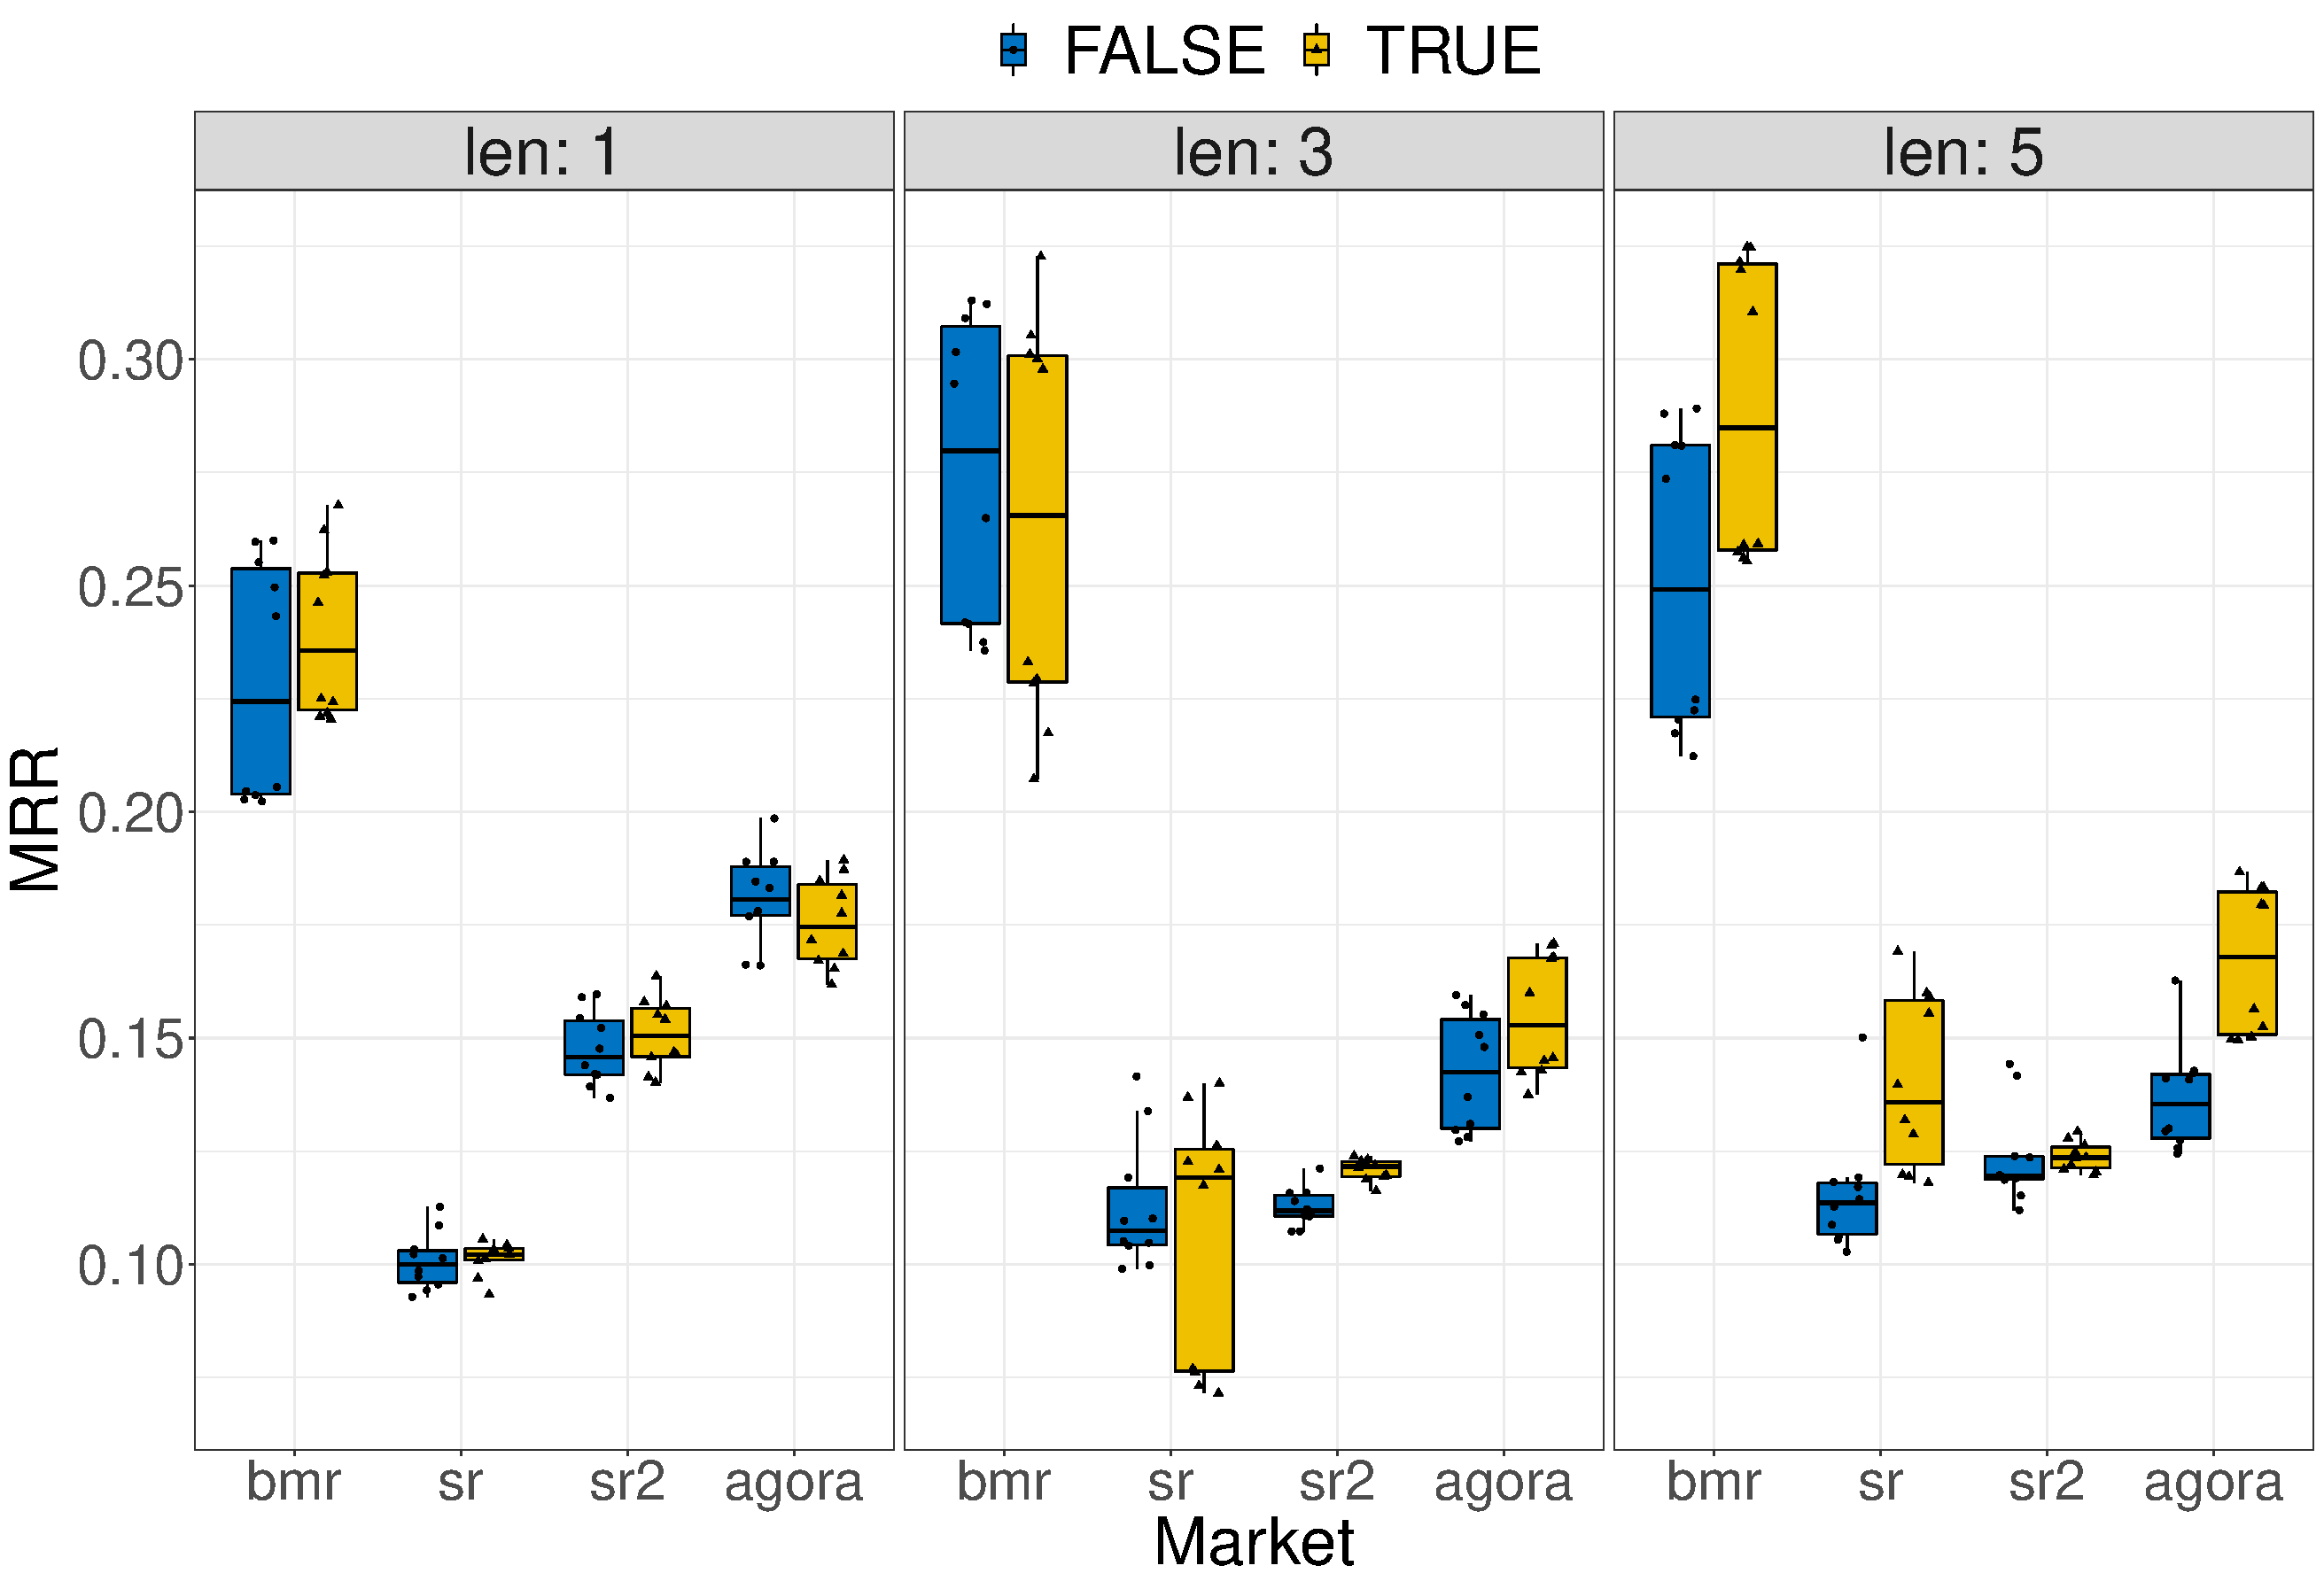
\includegraphics[width=\linewidth]{plots/graphemb_comparison.pdf}
        \caption{Graph Embedding}
        \label{fig:model_comp:graph}
    \end{subfigure} %
    \caption{Comparison of models across Tokenizer variants (top) and usage of graph embedding (bottom). TRUE/FALSE refer to whether the model is initialized with pretrained HIN context embeddings. \textcolor{blue}{SP: Is this figure particularly useful -- does it add to the accompanying text you have laid out w.r.t WMW test?}}
    \label{fig:model_comp}
\end{figure*}\textcolor{red}{replace Figure~\ref{fig:model_comp} with table}
\end{comment}
%Figure~\ref{fig:model_comp} demonstrates two of the modeling decisions - the choice of tokenizer and the impact of using pretrained graph embeddings.
%\noindent \textbf{Single Task Model} 
To compare the variants using statistical tests, we compute the MRR of the data grouped by market, episode length, tokenizer, and a graph embedding indicator.
This leaves a small number of samples for paired comparison between groups, which precludes making normality assumptions for a t-test. 
Instead, we applied the paired two-samples Wilcoxon-Mann-Whitney (WMW) test~\cite{mann1947test}.
The first key contribution of our model is the use of meta-graph embeddings for context. 
The WMW test demonstrates that using pretrained graph embeddings was significantly better than using random embeddings ($p < 0.01$). 
Table~\ref{tab:baselines_comparison} shows a summary of these results using ablations.
For completeness of the analysis, we also compare the character and BPE tokenizers.
WMW failed to find any significant differences between the BPE and character models for embedding (table omitted for brevity). 
Many darkweb markets tend to have more than one language (e.g., BMR had a large German community), and BPE  allows a shared vocabulary to be used across multiple datasets with very few out-of-vocab tokens. 
Thus, we use BPE tokens for the forthcoming multitask models.
\begin{figure}[!htbp]
    \centering
    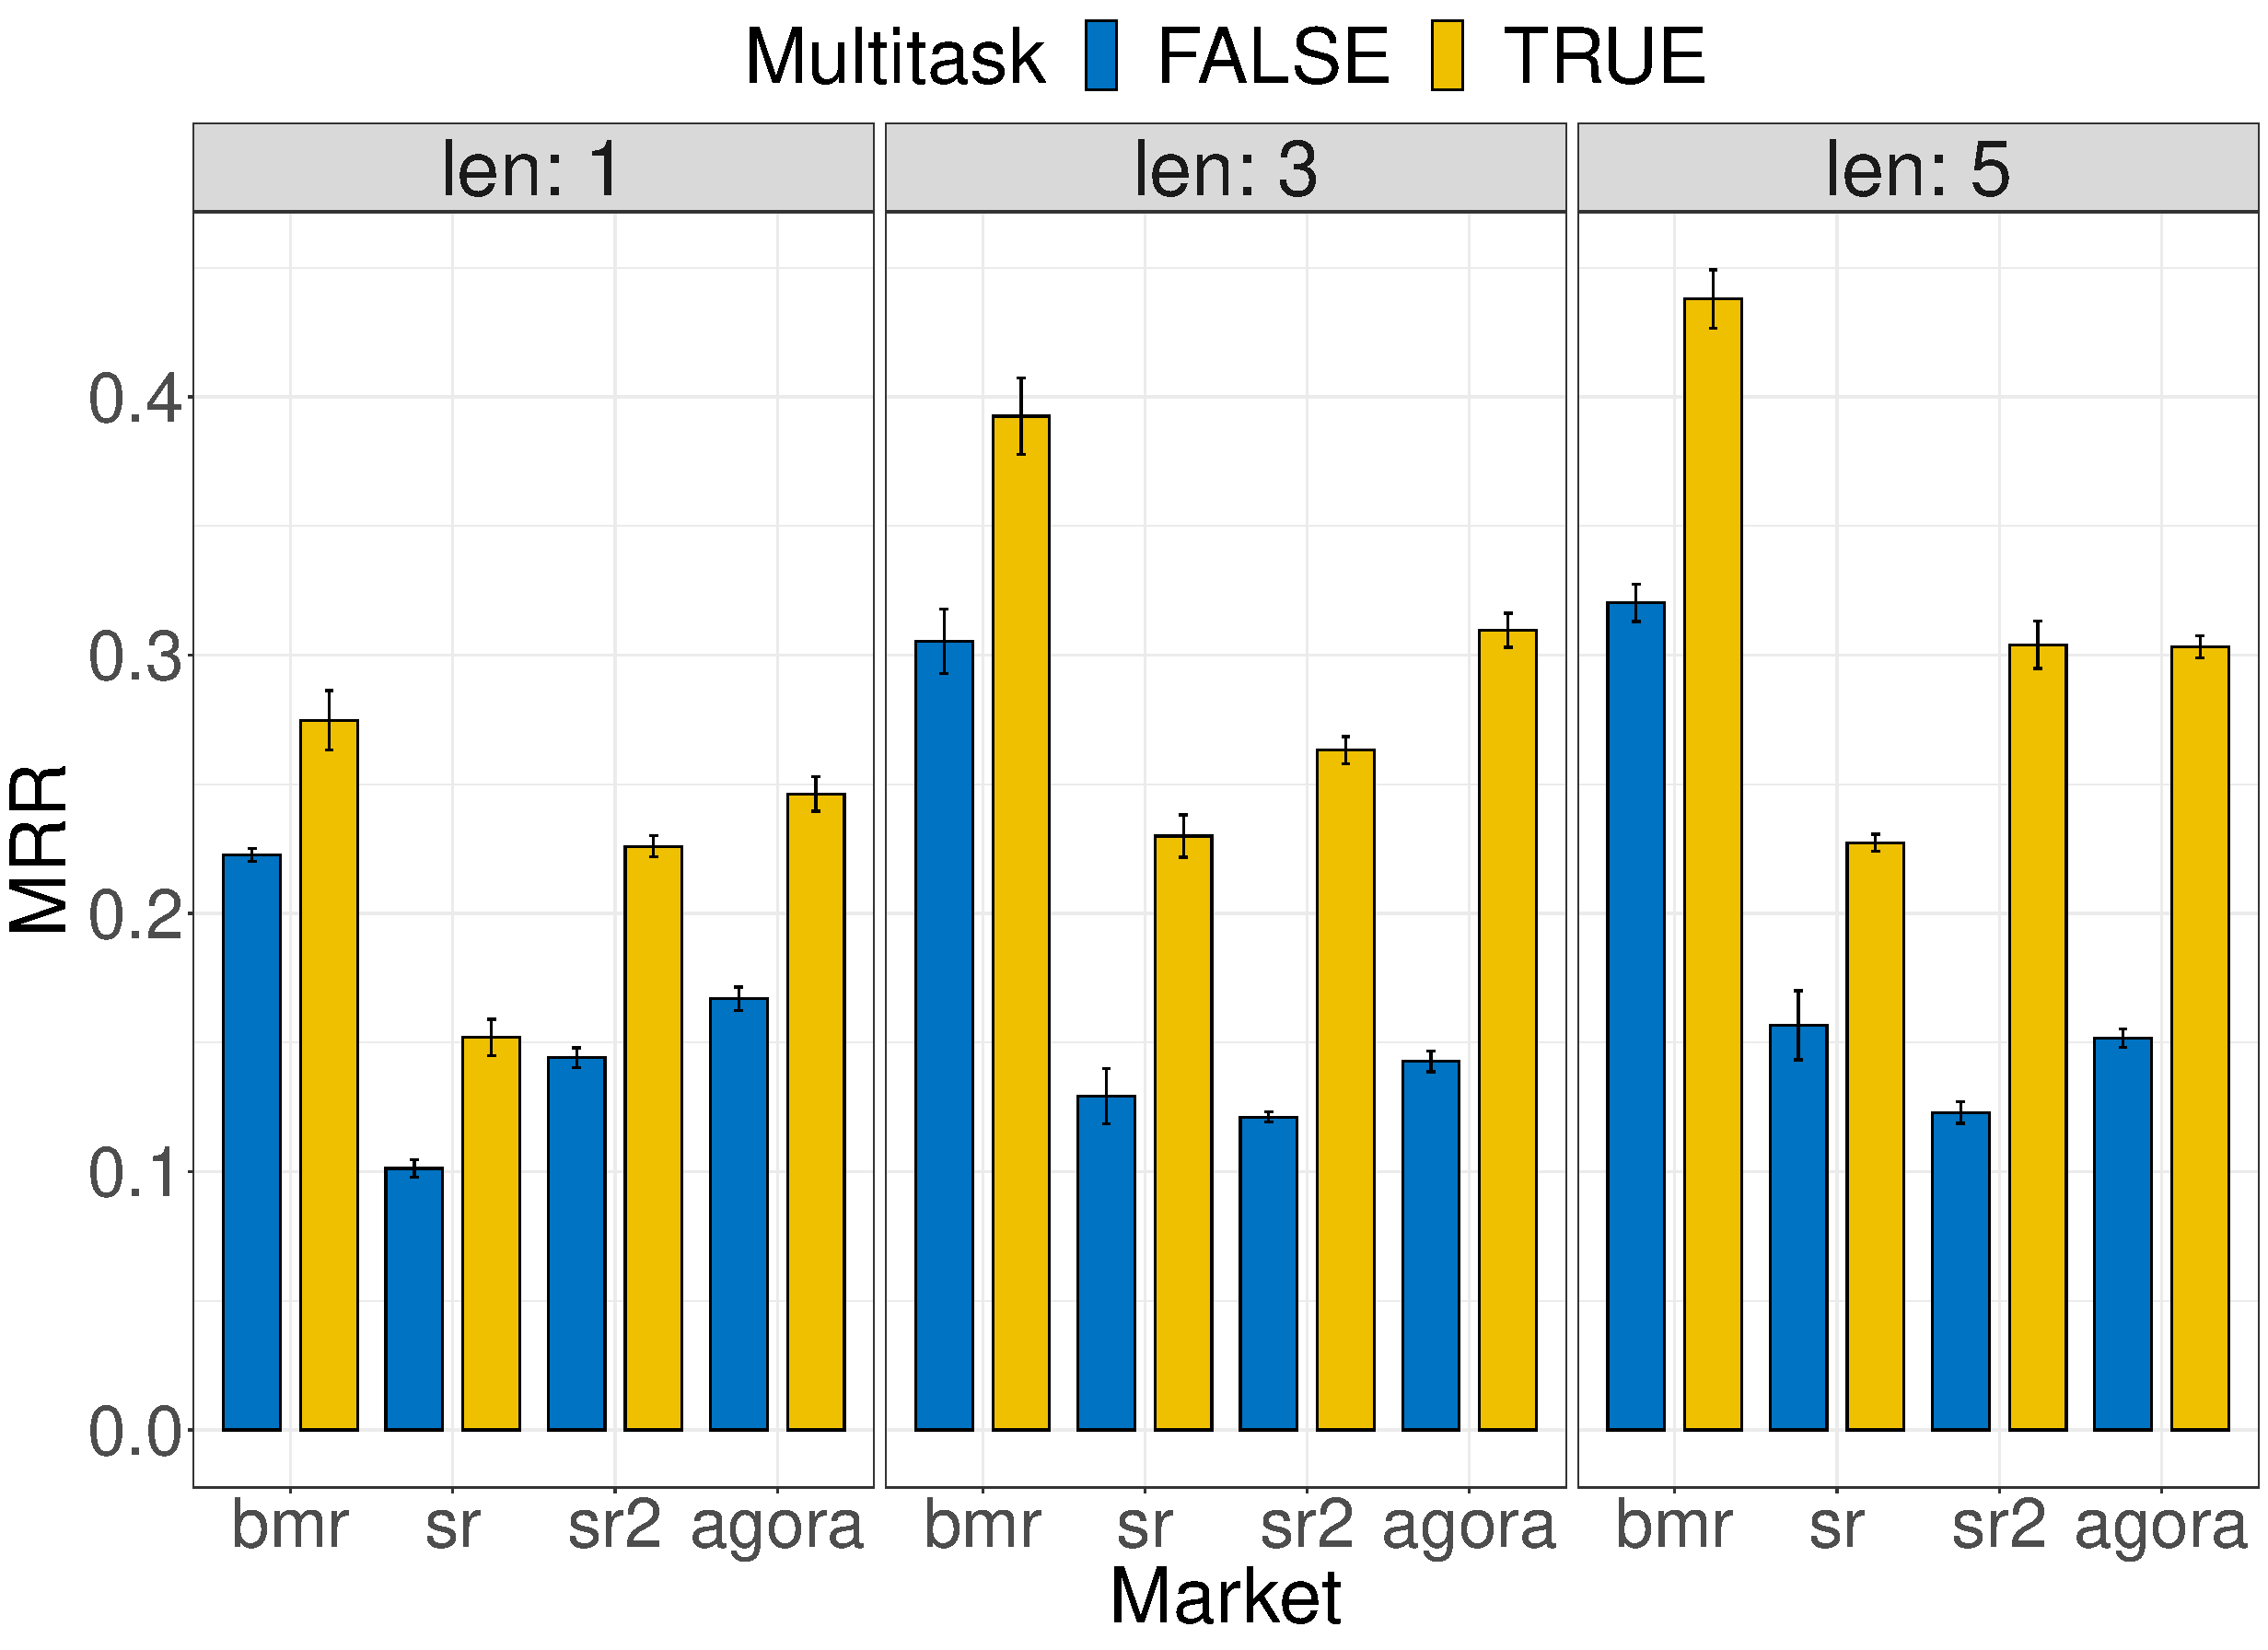
\includegraphics[width=0.8\linewidth,alt={Bar chart showing drill-down: one-at-a-time vs. multitask.}]{sysml/plots/multitask.pdf}
    \caption{Drill-down: one-at-a-time vs. multitask.}
    \label{fig:multitask_results}
\end{figure} 

\noindent \textbf{Multitask} Our second key contribution is the multitask setup.
Table~\ref{tab:baselines_comparison} demonstrates that \SYSMLmethodname{} (multitask) outperforms all baselines on episodes of length 5. We further compare runs of the best single task model for each market against a multitask model. %trained with $P(\text{cross\_sampling}) = 0.01$. 
Figure~\ref{fig:multitask_results} demonstrates that multitask learning  consistently and significantly (WMW: $p < 0.01$) improves performance across all markets and all episode lengths. 




\noindent \textbf{Metric Learning}
Recent benchmark evaluations have demonstrated that different metric learning methods provide only marginal improvements over classification~\cite{musgrave2020metric,Zhai2019ClassificationIA}. 
We experimented with various state-of-the-art metric learning methods (\S\ref{sec:framework:metric_learning}) in the multi task setup and found that softmax-based classification (SM) was the best performing method in 3 of 4 cases for episodes of length 5 (Figure~\ref{fig:metric_learning}). 
Across all lengths, SM is significantly better (WMW: $p < 1e-8$) and therefore we use SM in \SYSMLmethodname{}.

\begin{figure}[!htbp]
    \centering
    \includegraphics[width=0.8\linewidth,alt={Bar chart showing comparison of metric learning approaches.}]{sysml/plots/nce_comparison_multitask.pdf}
    \caption{Task comparison: SM and CF are better performing two methods, with SM better in 3 of 4 cases.}
    \label{fig:metric_learning}
\end{figure}
%\textcolor{red}{Consider dropping to single line}
%Recent benchmark evaluations have demonstrated that different metric learning methods provide only marginal improvements over classification~\cite{musgrave2020metric,Zhai2019ClassificationIA}. 
%We experimented with various state-of-the-art metric learning methods (\S\ref{sec:framework:metric_learning}) in the multi task setup and found that softmax-based classification (SM) was significantly better (WMW: $p < 0.01$). Therefore, we use SM in \SYSMLmethodname{}. 
%For additional details see the appendix.


\begin{comment}
\begin{figure}[!htbp]
    \centering
    \includegraphics[width=0.7\linewidth]{plots/nce_comparison_multitask.pdf}
    \caption{Task comparison: SM and CF are better performing two methods, with SM better in 3 of 4 cases.}
    \label{fig:metric_learning}
\end{figure}
\end{comment}

\begin{comment}
\noindent \textbf{Episode Length}  Figure~\ref{fig:len_comparison} shows a comparison of the mean performance of each model across various episode lengths. We see that compared to the baselines, \SYSMLmethodname{} can combine contextual and stylistic information across multiple posts more effectively. 

\begin{figure}[!htbp]
    \centering
    \includegraphics[width=0.7\linewidth]{plots/length_comparison.pdf}
    \caption{\SYSMLmethodname{} is more effective at utilizing multi post stylometric informatio.n}
    \label{fig:len_comparison}
\end{figure}
\end{comment}


\subsection{Novel Users}
The dataset statistics (Table~\ref{tab:dataset_stats}) indicate that there are users in each dataset who have no posts in the time period corresponding to the training data. 
To understand the distribution of performance across these two configurations, we compute the test metrics over two samples.
For one sample, we constrain the sampled episodes to those by users who have at least one episode in the training period (Seen Users).
For the second sample, we sample episodes from the complement of the episodes that satisfy the previous constraint (Novel Users).
Figure~\ref{fig:novel_vs_train_comparison} shows the comparison of MRR on these two samples against the best single task model for episodes of length 5. 
Unsurprisingly, the first sample (Seen Users) have better query metrics than the second (Novel Users).
However, importantly both of these groups outperformed the best single task model results on the first group (Seen Users), which demonstrates that the {\it lift offered by the multitask setup is spread across all users.} 

\begin{figure}
    \centering
    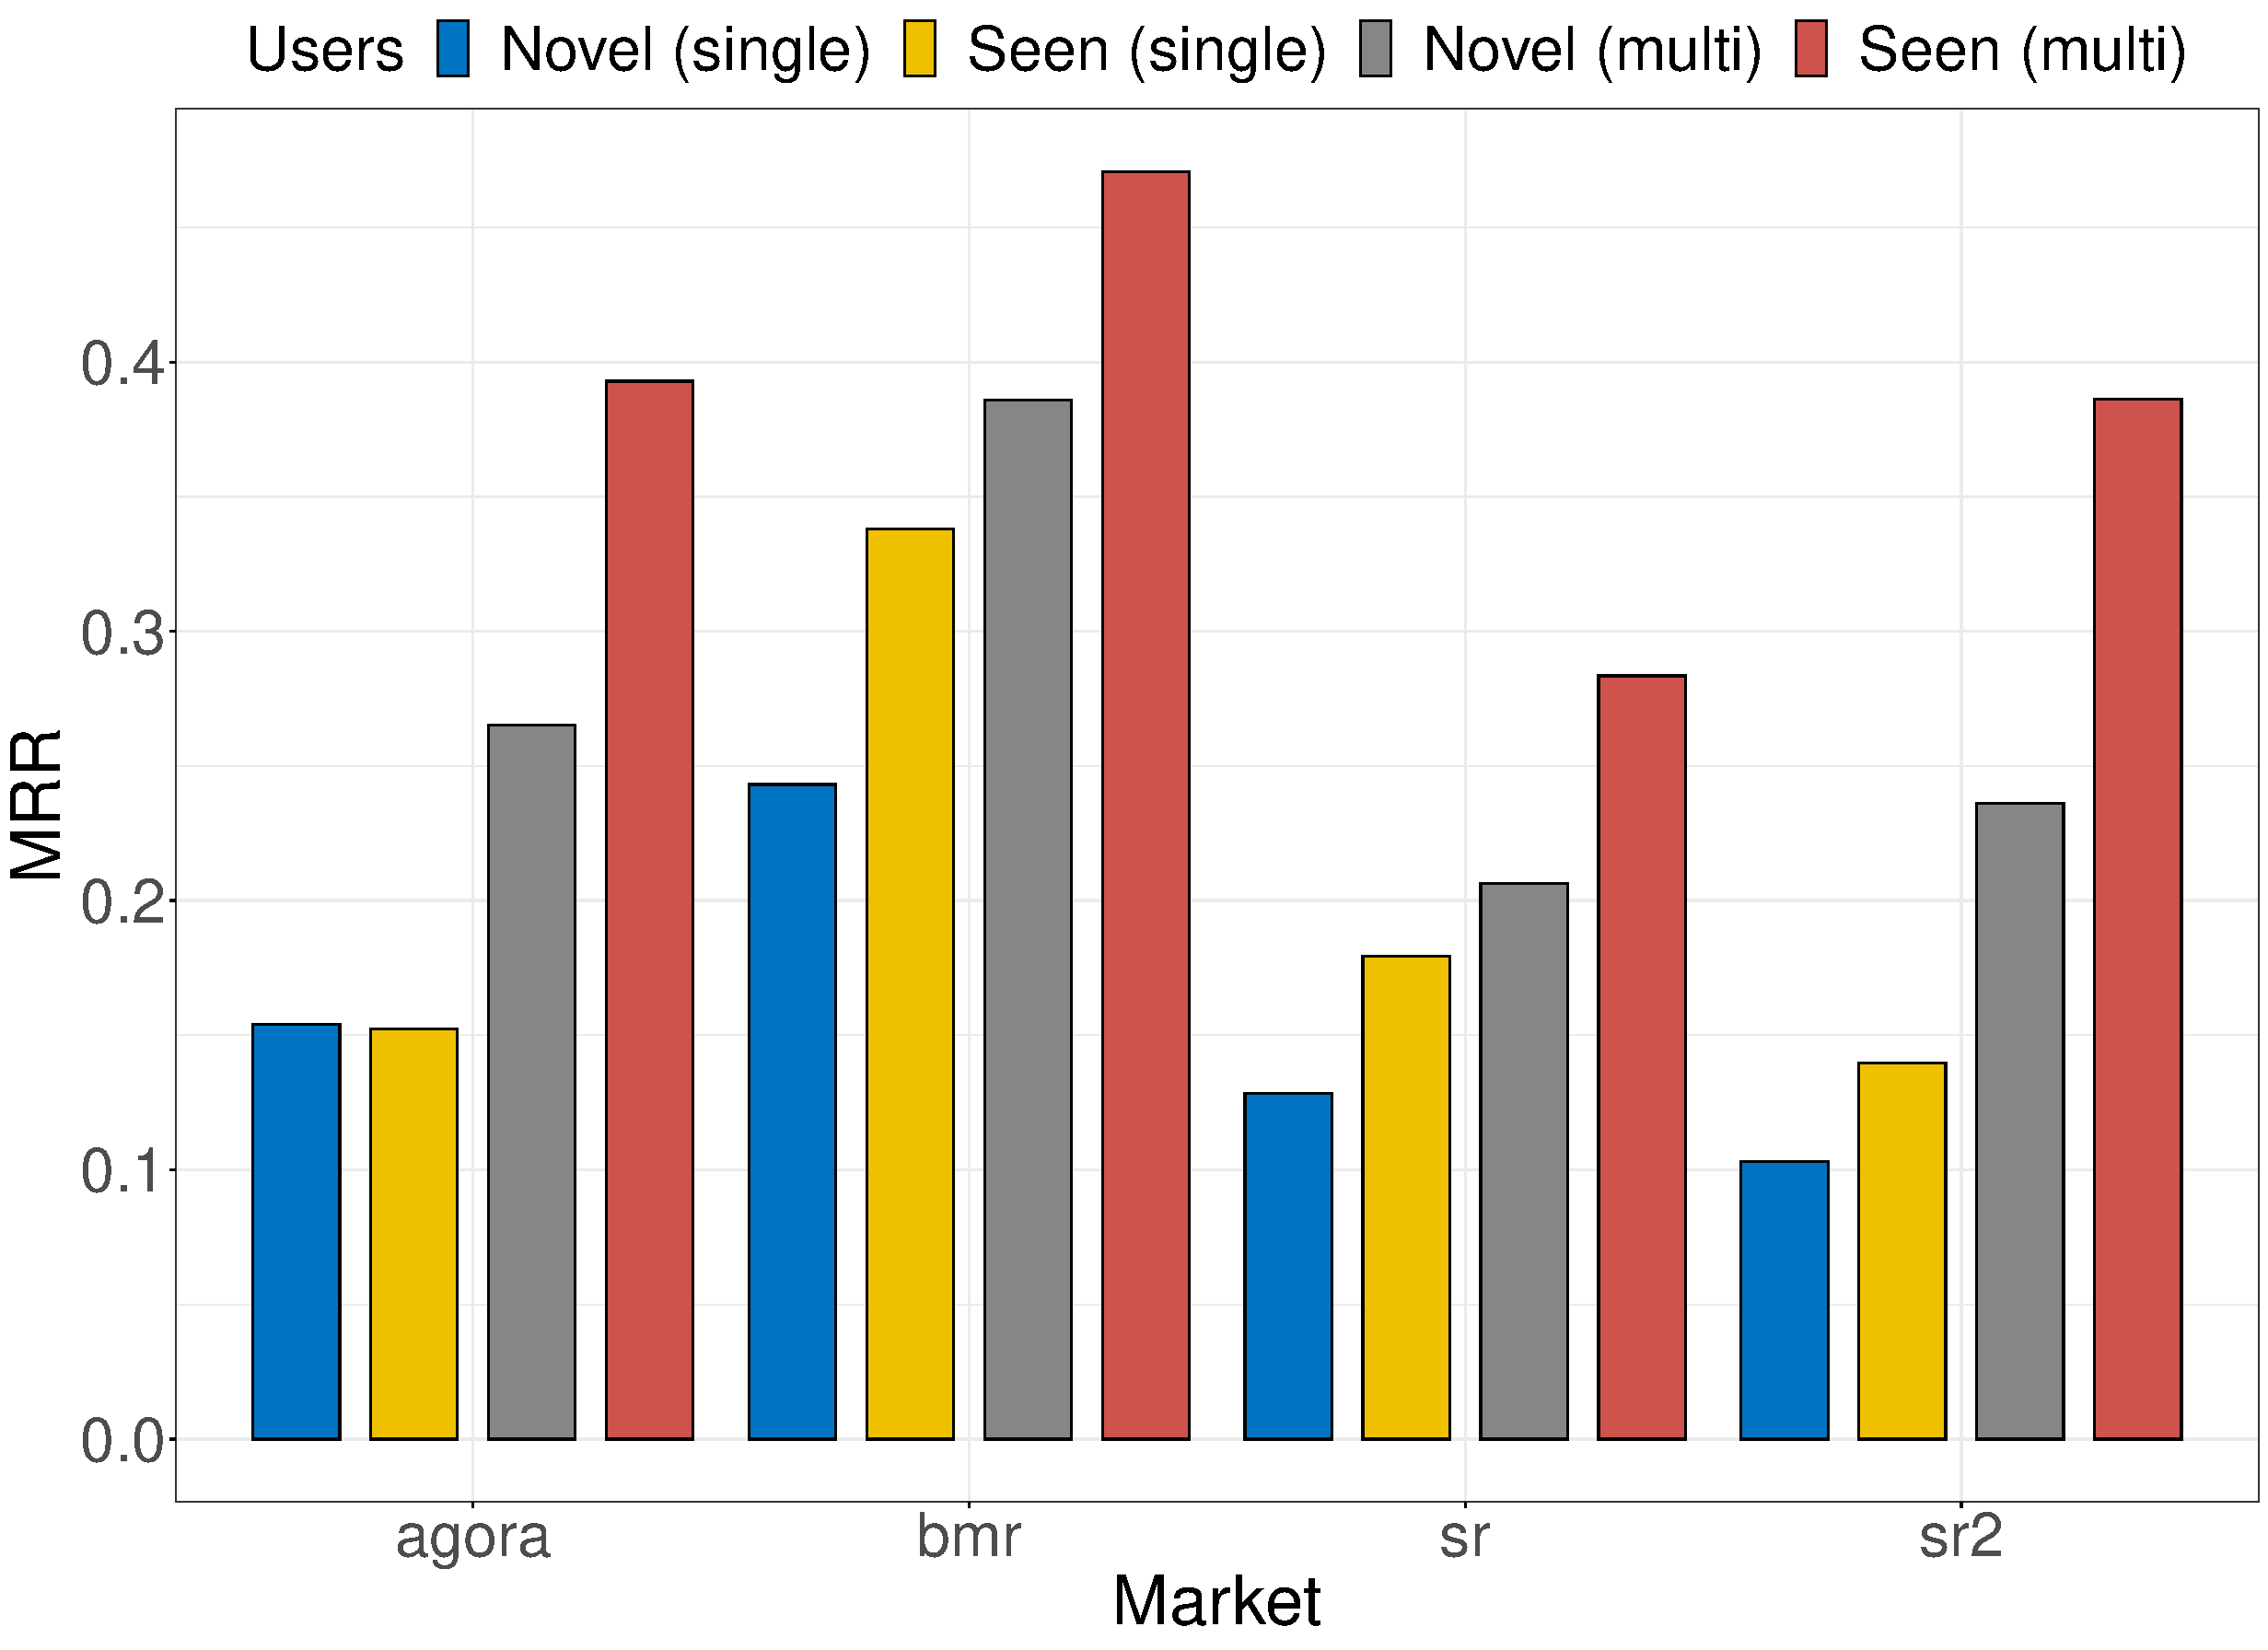
\includegraphics[width=0.8\linewidth,alt={Bar chart showing the lift provided by using the multitask setup across both seen and novel users.}]{sysml/plots/novel_vs_train_vs_single.pdf}
    \caption{Lift on the multitask setup across users.}
    \label{fig:novel_vs_train_comparison}
\end{figure}

\noindent \textbf{Episode Length}  Figure~\ref{fig:len_comparison} shows a comparison of the mean performance of each model across various episode lengths. We see that compared to the baselines, \SYSMLmethodname{} can combine contextual and stylistic information across multiple posts more effectively. Additional results (see appendix),  indicate that this trend continues for larger episode sizes.

\begin{figure}[!htbp]
    \centering
    \includegraphics[width=0.8\linewidth,alt={Line chart showing the improvements from \SYSMLmethodname{} across different episode lengths.}]{sysml/plots/length_comparison.pdf}
    \caption{\SYSMLmethodname{} is more effective at utilizing multi post stylometric information}
    \label{fig:len_comparison}
\end{figure}


\begin{figure}
    \centering
    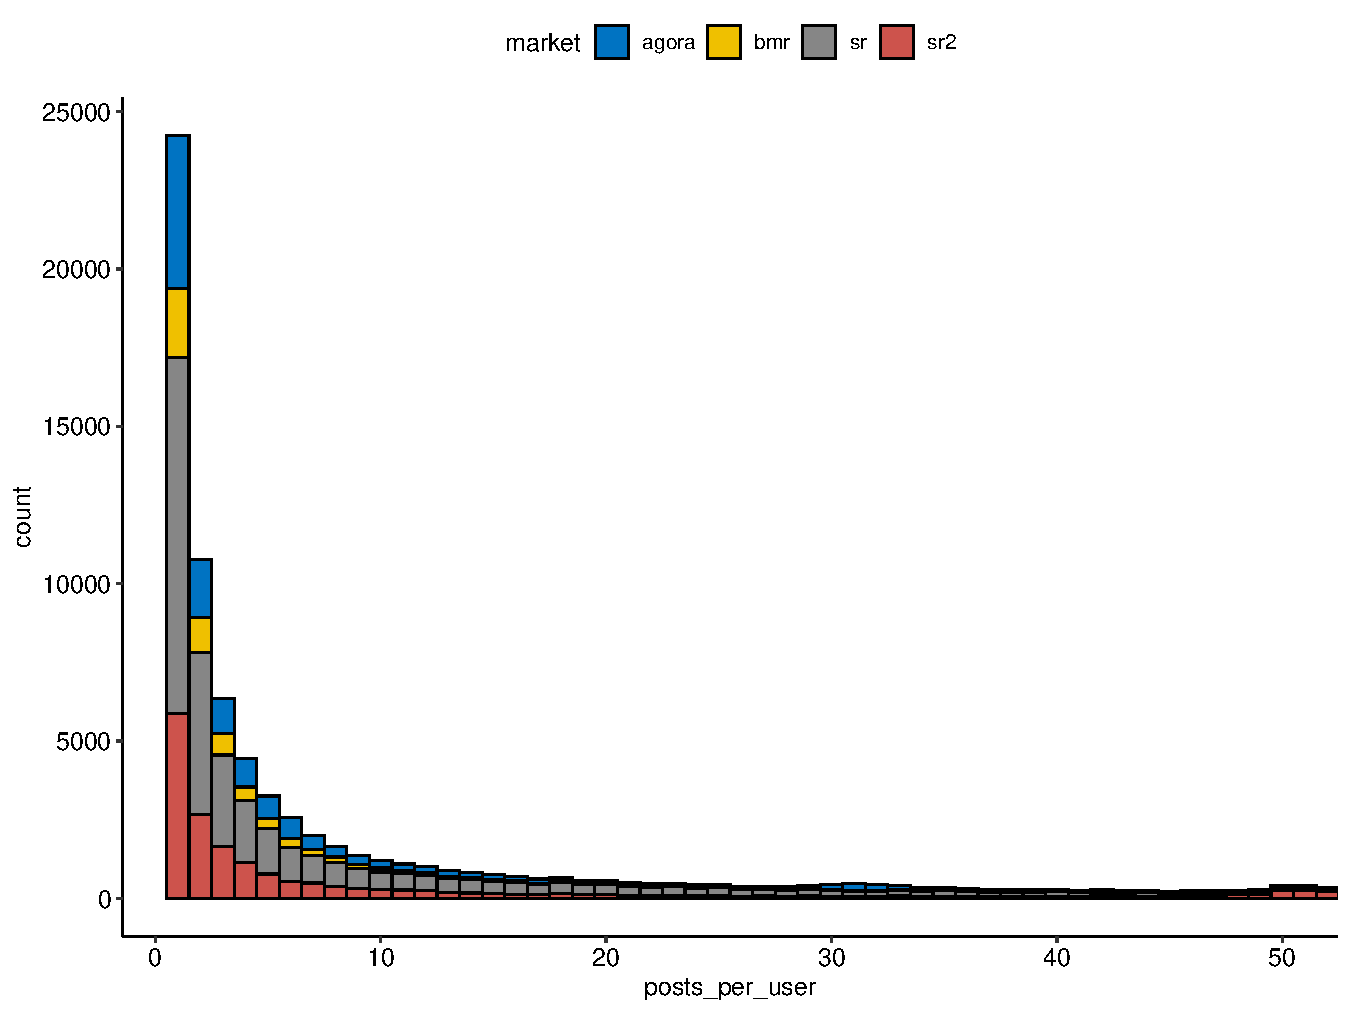
\includegraphics[width=\linewidth,alt={Histogram of posts per user.}]{sysml/plots/posts_histogram.pdf}
    \caption{Frequency of number of posts per user}
    \label{fig:posts_freq}
\end{figure}

\begin{table*}[!htbp]
    \small
    \centering
		\begin{tabular}{lcccccccc}
 		\toprule
			\multirow{2}{*}{Method}	&\multicolumn{2}{c}{BMR}	&	\multicolumn{2}{c}{Agora}	&	\multicolumn{2}{c}{SR2}	&	\multicolumn{2}{c}{SR}\\
					&MRR&	R@10&	MRR&	R@10&	MRR&	R@10&	MRR&	R@10\\
		\midrule
			\SYSMLmethodname{}  (singletask) &	0.305	&	0.508	&	0.186	&	0.32	&	0.159	&	0.273	&	0.14	&	0.246	\\
				\hline
			\SYSMLmethodname{}  (multitask) &	0.484	& 0.689	&	0.349	&	0.519	&	0.401	&	0.556	&	0.292	&	0.429	\\
					\bottomrule
    	\end{tabular}
    	\caption{Additional results for 7 posts per episode}
      \label{tab:additional_res_7}
\end{table*}

\begin{table*}[!htbp]
    \small
    \centering
		\begin{tabular}{lcccccccc}
 		\toprule
			\multirow{2}{*}{Method}	&\multicolumn{2}{c}{BMR}	&	\multicolumn{2}{c}{Agora}	&	\multicolumn{2}{c}{SR2}	&	\multicolumn{2}{c}{SR}\\
					&MRR&	R@10&	MRR&	R@10&	MRR&	R@10&	MRR&	R@10\\
		\midrule
			\SYSMLmethodname{}  (singletask) &	0.264 & 0.48	&	0.146	&	0.249	&	0.165   &	0.272	&	0.194	&	0.319	\\
				\hline
			\SYSMLmethodname{}  (multitask) &	0.4667	&	 0.648	&	0.357	&	0.498	&	0.377	&	0.522	&	0.299	&	0.449	\\
					\bottomrule
    	\end{tabular}
    	\caption{Additional results for 9 posts per episode}
      \label{tab:additional_res_9}
\end{table*}

From Figure~\ref{fig:posts_freq}, we see that the number of users reduces rapidly as the posts per user decrease. Thus, we limited our analysis to up to 5 posts per episode.
For completeness, we also provide additional results for 7 and 9 posts per episode in Table~\ref{tab:additional_res_7} and ~\ref{tab:additional_res_9} respectively. Note that the histogram has some non-smooth bumps at around 10, 50, 100 posts as they act as the minimum number of posts for different levels of forum users. As explained in a previous section, users post on `newbie' forums until they reach a specific number of posts, leading to these unusual bumps in the histogram. 
We note that the performance of our methods continues to improve as the posts per episode are increased (at a cost to coverage - number of users studied), though the improvement is higher in the bigger markets as these tend to have a sufficiently large number of individuals with a higher number of total posts.
